\documentclass[UTF8,12pt]{article}
\usepackage{ctex}
\usepackage{indentfirst}
\usepackage{color}
\usepackage{hyperref}
\usepackage{graphicx}
\usepackage{subfigure}
\usepackage{pdfpages}
\usepackage{listings}
\usepackage{afterpage}
\usepackage{geometry}
\usepackage{booktabs}
\usepackage{multirow}
\usepackage{graphicx}

\geometry{a4paper,scale=0.8}

\newcommand\myemptypage{
    \null
    \thispagestyle{empty}
    \addtocounter{page}{-1}
    \newpage
}

\hypersetup{
    hidelinks,
	colorlinks=true,
	allcolors=black,
	pdfstartview=Fit,
	breaklinks=true
}

\definecolor{dkgreen}{rgb}{0,0.6,0}
\definecolor{gray}{rgb}{0.5,0.5,0.5}
\definecolor{mauve}{rgb}{0.58,0,0.82}

\lstset{ %
  language=Octave,                % the language of the code
  basicstyle=\footnotesize,           % the size of the fonts that are used for the code
  numbers=left,                   % where to put the line-numbers
  numberstyle=\tiny\color{gray},  % the style that is used for the line-numbers
  stepnumber=2,                   % the step between two line-numbers. If it's 1, each line 
                                  % will be numbered
  numbersep=5pt,                  % how far the line-numbers are from the code
  backgroundcolor=\color{white},      % choose the background color. You must add \usepackage{color}
  showspaces=false,               % show spaces adding particular underscores
  showstringspaces=false,         % underline spaces within strings
  showtabs=false,                 % show tabs within strings adding particular underscores
  frame=single,                   % adds a frame around the code
  rulecolor=\color{black},        % if not set, the frame-color may be changed on line-breaks within not-black text (e.g. commens (green here))
  tabsize=2,                      % sets default tabsize to 2 spaces
  captionpos=b,                   % sets the caption-position to bottom
  breaklines=true,                % sets automatic line breaking
  breakatwhitespace=false,        % sets if automatic breaks should only happen at whitespace
  title=\lstname,                   % show the filename of files included with \lstinputlisting;
                                  % also try caption instead of title
  keywordstyle=\color{blue},          % keyword style
  commentstyle=\color{dkgreen},       % comment style
  stringstyle=\color{mauve},         % string literal style
  escapeinside={\%*}{*)},            % if you want to add LaTeX within your code
  morekeywords={*,...}               % if you want to add more keywords to the set
}


\setlength{\parindent}{2em}

\begin{document}

\begin{titlepage}
    \includepdf[pages={1}]{cover2.pdf}
\end{titlepage}

\myemptypage

\begin{center}
    \tableofcontents
\end{center}

\newpage

% 一、实验目的
% 指出此次实验应该达到的学习目标。
% 二、实验内容
% 指出此次实验应完成的任务。
% 三、实验方法
% 包括实验方法、原理、技术、方案等。
% 四、实验步骤
% 指出完成该实验的操作步骤。
% 五、实验结果
% 记录实验输出数据和结果。
% 六、实验结论
% 对实验数据和结果进行分析描述,给出实验取得的成果和结论。
% 注:有程序的要求附上程序源代码,有图表的要有截图并有相应的文字说明和分析
% 七、实验小结
% 给出本次实验的体会,如学会了什么,遇到哪些问题,如何解决这些问题,存在哪些有待改进的地方。

实验学时:2

每组人数:3

实验类别:2\ (1:基础性\ 2:综合性\ 3:设计性\ 4:研究性)

实验要求:1\ (1:必修\ 2:选修\ 3:其它)

实验类别:3\ (1:基础\ 2:专业基础\ 3:专业\ 4:其它)

\section{实验目的}
\begin{itemize}
  \item 掌握外部中断的处理流程;
  \item 掌握Cortex-M7处理器的中断方式和中断处理过程;
  \item 通过实验学习Cortex-M7处理器的中断响应流程;
  \item 通过实验掌握Cortex-M7处理器中断处理的软件编程方法;
  \item 通过实验掌握Cortex-M7处理器中断响应过程中相关寄存器的使用方法。
\end{itemize}

\section{实验内容}
编写程序,对指定GPIO端口进行初始化,完成外部中断相关寄存器的配置,使用ARM Cortex-M7实验平台的按键S3产生外部中断,在中断响应过程中对LED进行控制,并采用不同的中断设置方法实现多种中断触发方式。实验过程中观察上升沿触发选择寄存器(EXTI\_RTSR)和下降沿触发选择寄存器(EXTI\_FTSR)的值对中断触发条件的影响,学习Cortex-M7外部中断线的设置方法和初始化,以及外部中断的触发方式和响应过程。

\section{实验方法}
\subsection{实验原理}
\begin{enumerate}
  \item STM32F746NG的外部中断和事件控制器(EXTI)
  
  STM32F746NG具有多达24个用于产生中断/事件请求的边沿检测器(输入线)。每根输入线都可以单独进行配置,以选择类型(中断或事件)和响应的触发事件(上升沿触发、下降沿触发或边沿触发),每根输入线还可以单独屏蔽。挂起寄存器用于保持中断请求。
  EXTI控制器的主要特性如下:
  \begin{itemize}
    \item 每个中断/事件线上都具有独立的触发和屏蔽;
    \item 每个中断线具有专用的状态位;
    \item 支持多大24个软件事件/中断请求;
    \item 检测脉冲宽度低于APB2时钟宽度的外部信号。
  \end{itemize}
  要产生中断,必须先配置好并使能中断线。根据需要的边沿检测设置2个触发寄存器,同时在中断屏蔽寄存器的相应位写“1”使能中断请求。当外部中断线上出现选定信号沿时,便会产生中断请求,对应的挂起位也会置1。在挂起寄存器的对应位写“1”,将清除该中断请求。
  要产生事件,必须先配置好并使能事件线。根据需要的边沿检测设置2个触发寄存器,同时在事件屏蔽寄存器的相应位写“1”使能事件请求。当事件线上出现选定信号沿时,便会产生事件脉冲,对应的挂起位会置1。
  通过在软件中对中断/事件寄存器写“1”,也可以产生中断/事件请求。
  要将一根输入线配置为中断源,需执行以下步骤:
  \begin{enumerate}
    \item 配置相应的屏蔽位(EXTI\_IMR);
    \item 配置中断线的触发选择位(EXTI\_RTSR和EXTI\_FTSR);
    \item 配置对应到外部中断控制器(EXTI)的NVIC中断通道的使能和屏蔽位,使得24个中断线中的请求可以被正确的响应。
  \end{enumerate}
  要将一根输入线配置为事件源,需执行以下步骤:
  \begin{enumerate}
    \item 配置相应的屏蔽位(EXTI\_EMR);
    \item 配置事件线的触发选择位(EXTI\_RTSR和EXTI\_FTSR);
  \end{enumerate}
  \item 外部中断/事件线映射及控制器框图
  
  如图所示,多达168个GPIO通过图中方式连接到16个外部中断/事件线。
  \begin{figure}[htbp]
    \centering
    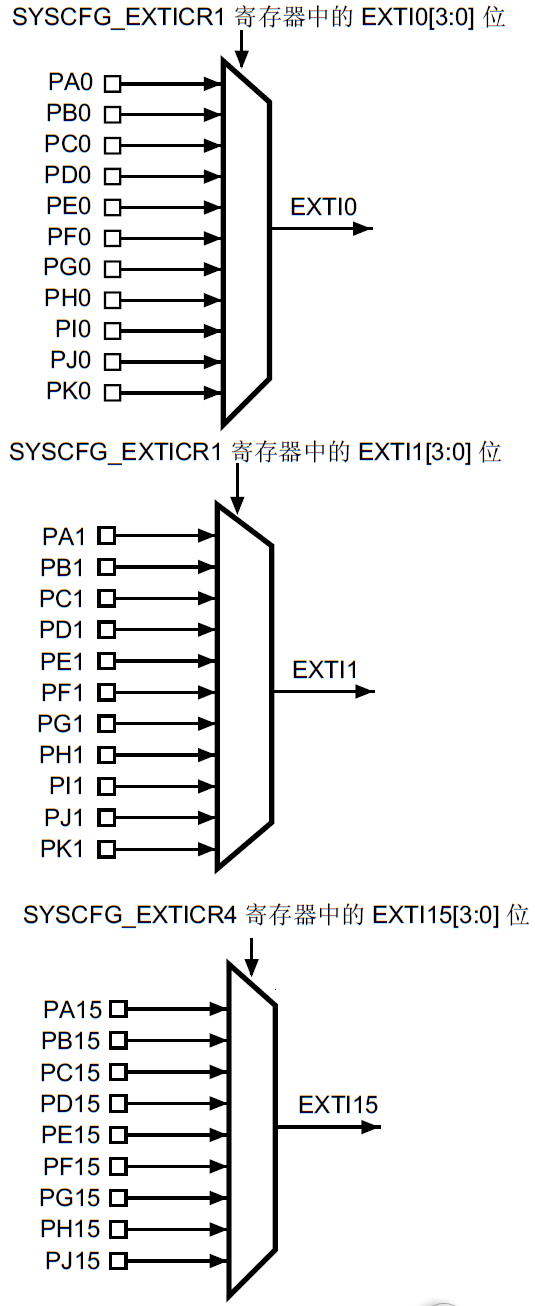
\includegraphics[width=0.3\textwidth]{imgs/3.png}
    \caption{外部中断/事件GPIO映射}
  \end{figure}
  另外8根EXTI线连接方式如下:
  \begin{itemize}
    \item EXTI16连接到PVD输出;
    \item EXTI17连接到RTC闹钟事件;
    \item EXTI18连接到USB OTG FS唤醒事件;
    \item EXTI19连接到以太网唤醒事件;
    \item EXTI20连接到USB OTG HS唤醒事件
    \item EXTI21连接到RTC侵入和时间戳事件
    \item EXTI22连接到RTC唤醒事件;
    \item EXTI23连接到LPTIM1异步事件。
  \end{itemize}
  EXTI控制器框图如图所示
  \begin{figure}[htbp]
    \centering
    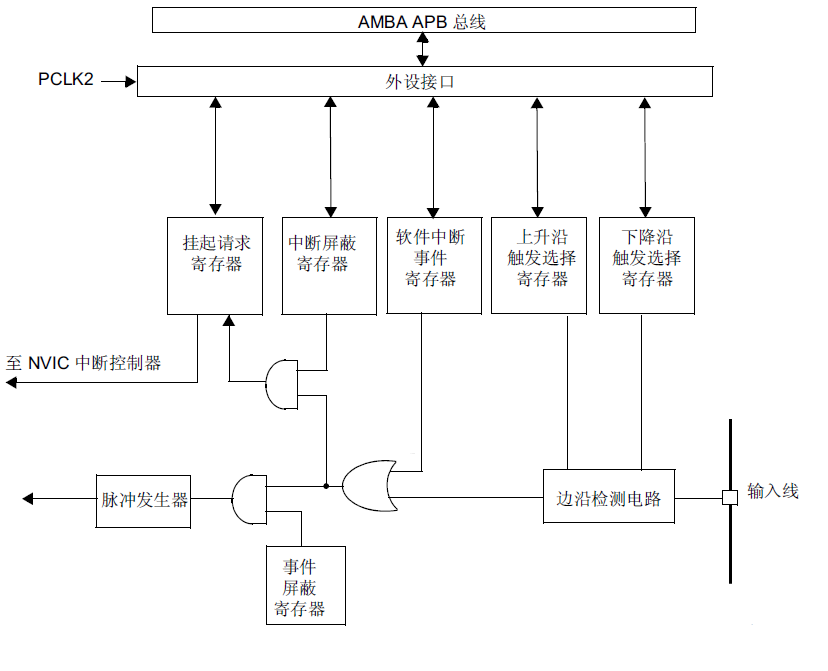
\includegraphics[width=0.3\textwidth]{imgs/4.png}
    \caption{EXTI控制器框图}
  \end{figure}

  \item EXTI寄存器
  
  \begin{enumerate}
    \item 中断屏蔽寄存器(EXTI\_IMR)
    
    偏移地址:0x00

    复位值:0x0000 0000

    中断屏蔽寄存器如图所示
    \begin{figure}[htbp]
      \centering
      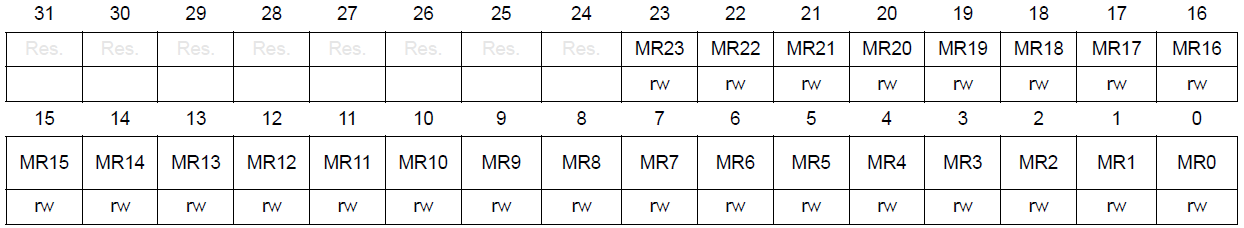
\includegraphics[width=0.8\textwidth]{imgs/5.png}
      \caption{中断屏蔽寄存器}
    \end{figure}

    位31:24保留,必须保持复位值。

    MRx:x线上的中断屏蔽

    0:屏蔽来自x线的中断请求

    1:开放来自x线的中断请求

    \item 事件屏蔽寄存器(EXTI\_EMR)
    
    偏移地址:0x04

    复位值:0x0000 0000

    事件屏蔽寄存器如图所示。

    \begin{figure}[htbp]
      \centering
      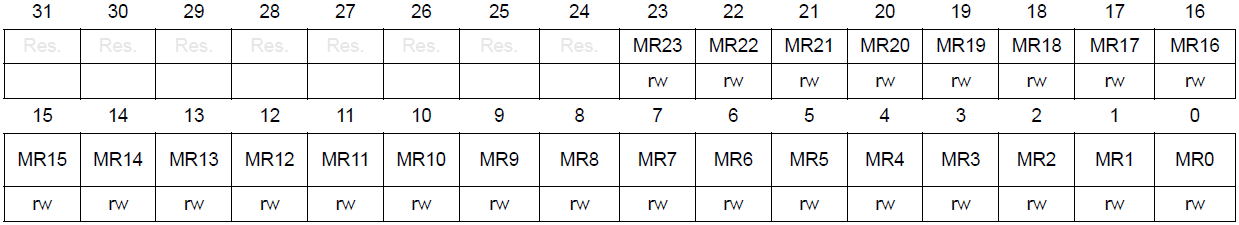
\includegraphics[width=0.8\textwidth]{imgs/6.png}
      \caption{事件屏蔽寄存器}
    \end{figure}

    位31:24保留,必须保持复位值。

    MRx:x线上的事件屏蔽

    0:屏蔽来自x线的事件请求

    1:开放来自x线的事件请求

    \item 上升沿触发选择寄存器(EXTI\_RTSR)
    
    偏移地址:0x08

    复位值:0x0000 0000

    上升沿触发选择寄存器如图所示。

    \begin{figure}[htbp]
      \centering
      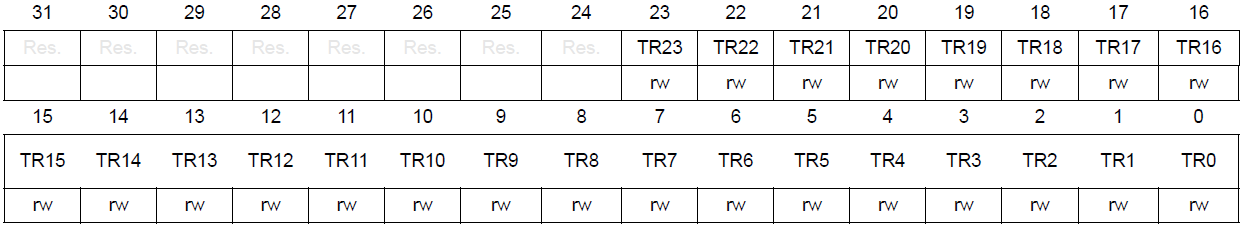
\includegraphics[width=0.8\textwidth]{imgs/7.png}
      \caption{上升沿触发选择寄存器}
    \end{figure}

    位31:24保留,必须保持复位值。

    TRx:x线的上升沿触发事件配置位

    0:禁止输入线上升沿触发(事件和中断)

    1:开放输入线上升沿触发(事件和中断)

    注:外部唤醒线配置为边沿触发时,在这些线上不能出现毛刺信号。
    
    如果在向EXTI\_RTSR寄存器写入值的同时外部中断线上产生上升沿,挂起位将被置位。
    
    在同一中断线上,可以同时设置上升沿和下降沿触发,即任一边沿都可触发中断。

    \item 下降沿触发选择寄存器(EXTI\_FTSR)
    
    偏移地址:0x0C

    复位值:0x0000 0000

    下降沿触发选择寄存器如图所示。

    \begin{figure}[htbp]
      \centering
      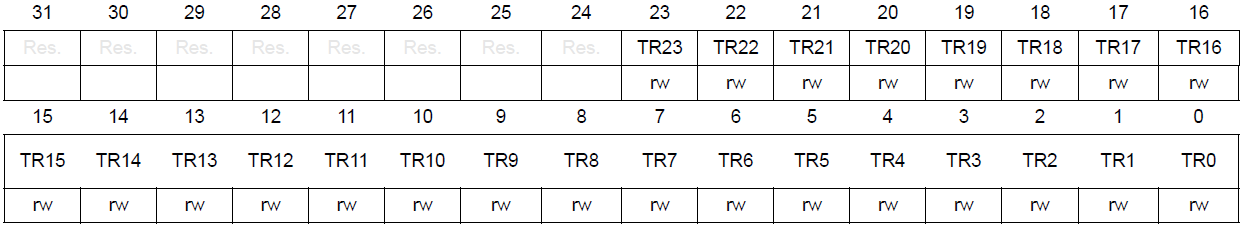
\includegraphics[width=0.8\textwidth]{imgs/8.png}
      \caption{下降沿触发选择寄存器}
    \end{figure}

    位31:24保留,必须保持复位值。

    TRx:x线的下降沿触发事件配置位

    0:禁止输入线下降沿触发(事件和中断)

    1:开放输入线下降沿触发(事件和中断)

    注:外部唤醒线配置为边沿触发时,在这些线上不能出现毛刺信号。

    如果在向EXTI\_FTSR寄存器写入值的同时外部中断线上产生下降沿,挂起位将被置位。

    在同一中断线上,可以同时设置上升沿和下降沿触发,即任一边沿都可触发中断。
    
    \item 软件中断事件寄存器(EXTI\_SWIER)
    
    偏移地址:0x10

    复位值:0x0000 0000

    软件中断事件寄存器如图所示。

    \begin{figure}[htbp]
      \centering
      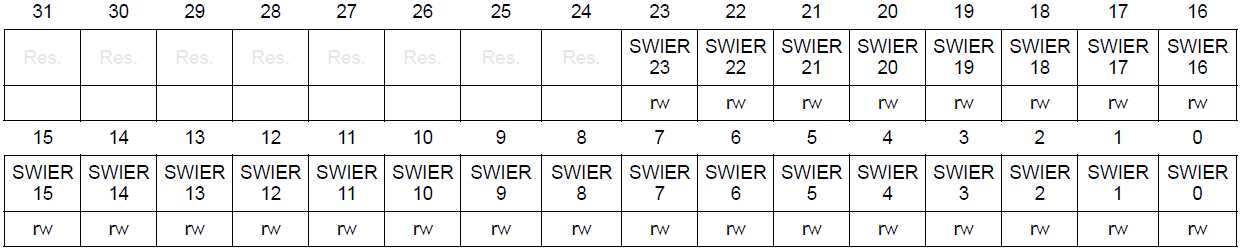
\includegraphics[width=0.8\textwidth]{imgs/9.png}
      \caption{软件中断事件寄存器}
    \end{figure}

    位31:24保留,必须保持复位值。

    SWIERx:x线的软件中断

    当SWIERx位设置为“0”时,将“1”写入该位会将EXTI\_PR寄存器中相应挂起位置1。如果在EXTI\_IMR寄存器中允许在x线上产生该中断,则产生中断请求。通过清除EXTI\_PR的对应位(写入“1”),可以清除该位为“0”。

    \item 挂起寄存器(EXTI\_PR)
    
    偏移地址:0x14

    复位值:未定义

    挂起寄存器如图所示。

    \begin{figure}[htbp]
      \centering
      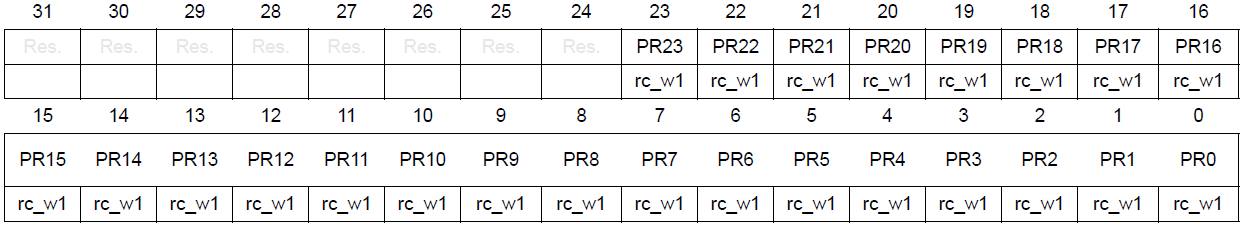
\includegraphics[width=0.8\textwidth]{imgs/10.png}
      \caption{挂起寄存器}
    \end{figure}

    位31:24保留,必须保持复位值。

    PRx:x线的挂起

    0:未发生触发请求

    1:发生了选择的触发请求

    注:当在外部中断线上发生了选择的边沿事件,该位被置1,将此位编程为“1”可清除此位。
  \end{enumerate}

  \item EXTI寄存器边界地址
  
  EXTI寄存器边界地为0x4001 3C00 – 0x4001 3FFF。

  \item 实验电路
  
  如图所示

  \begin{figure}[htbp]
    \centering
    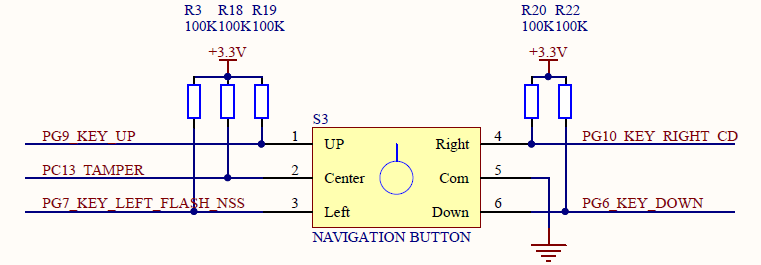
\includegraphics[width=0.8\textwidth]{imgs/11.png}
    \caption{实验电路}
  \end{figure}

  如图中所示,STM32F746芯片的PC13外接上拉电路,串联开关S3的Center(对应五向导航键S3的确定功能)后接地。由于I/O口外接上拉电路,所以在对I/O口进行初始化时可设置为浮空输入。开关S3断开时,PC13输入高电平;反之,PC13输入低电平。所以,当按下开关S3时,PC13输入由高变低,产生一个下降沿;当释放开关S3时,PC13输入由低变高,产生一个上升沿。根据外部中断触发条件设置,当满足所需的边沿条件时,触发中断,MCU响应中断点亮/熄灭发光二极管D1。
\end{enumerate}

\subsection{试验方案及调试过程}
\noindent
\textbf{基础实验}:本实验的实验例程(STM32F746\_Experiment\_v1.1/03\_EXTI)

实验例程如下:

\begin{lstlisting}[frame=shadowbox]
/**
  主程序:系统上电初始化后对LED1进行初始化,配置PC13作为外部中断源并开启中断,产生中断后点亮/熄灭LED。
**/
#include "main.h"
#include "system_init.h"

void System_Init(void);
void EXTI15_10_IRQHandler_Config(void);

/* main */
int main(void)
{
  System_Init();
  
  /* Initialize LED1 mounted on board */
  BSP_LED_Init(LED1);
  
  /* Configure EXTI15_10 (connected to PC.13 pin) in interrupt mode */
  EXTI15_10_IRQHandler_Config();
  
  while (1)
  {
  }
}

/* EXTI line detection callbacks, GPIO_Pin: Specifies the pins connected EXTI line */
void HAL_GPIO_EXTI_Callback(uint16_t GPIO_Pin)			//此处定义了HAL_GPIO_EXTI_Callback函数,原使用__weak  定义的函数被忽略�
{
  if (GPIO_Pin == GPIO_PIN_13)
  {
    /* Toggle LED1 */
    BSP_LED_Toggle(LED1);
    
    printf("\n\rLED1 switched\n\r");
  }
}
\end{lstlisting}
调试过程分析如下:

首先调用System\_Init()函数进行系统初始化,内部函数内容与实验一相同,不再赘述。

然后调用BSP\_LED\_Init()函数对LED1进行初始化,函数初始化板载LED1,使能LED1使其工作调用

\begin{lstlisting}[frame=shadowbox]
void BSP_LED_Init(Led_TypeDef Led)
{
  GPIO_InitTypeDef  gpio_init_structure;
  GPIO_TypeDef*     gpio_led;
	//Actualy only one LED
	switch(Led)
	{
		case LED1:
			/* Enable the GPIO_LED clock */
      LED1_GPIO_CLK_ENABLE();
			gpio_led = LED1_GPIO_PORT;
			break;
		case LED2:
			/* Enable the GPIO_LED clock */
      LED2_GPIO_CLK_ENABLE();
			gpio_led = LED2_GPIO_PORT;
			break;
		case LED3:
			/* Enable the GPIO_LED clock */
      LED3_GPIO_CLK_ENABLE();
			gpio_led = LED3_GPIO_PORT;
			break;
		case LED4:
			/* Enable the GPIO_LED clock */
      LED4_GPIO_CLK_ENABLE();
			gpio_led = LED4_GPIO_PORT;
			break;
		default:
			break;
	}
	/* Configure the GPIO_LED pin */
	gpio_init_structure.Pin = GPIO_PIN[Led];
	gpio_init_structure.Mode = GPIO_MODE_OUTPUT_PP;
	gpio_init_structure.Pull = GPIO_PULLUP;
	gpio_init_structure.Speed = GPIO_SPEED_HIGH;

	HAL_GPIO_Init(gpio_led, &gpio_init_structure);
	
	/* By default, turn off LED */
	HAL_GPIO_WritePin(gpio_led, GPIO_PIN[Led], GPIO_PIN_SET);
}
\end{lstlisting}
接着通过EXTI15\_10\_IRQHandler\_Config()函数配置PC13作为外部中断源并开启中断。

\begin{lstlisting}[frame=shadowbox]
void EXTI15_10_IRQHandler_Config(void)
{
  GPIO_InitTypeDef   GPIO_InitStructure;

  /* Enable GPIOC clock */
  __HAL_RCC_GPIOC_CLK_ENABLE();
	
  /* Configure PC.13 pin as input floating */
  GPIO_InitStructure.Mode = GPIO_MODE_IT_FALLING;				// 中断触发方式:下降沿触发
  GPIO_InitStructure.Pull = GPIO_NOPULL;								// GPIO内部无上拉或下拉
  GPIO_InitStructure.Pin = GPIO_PIN_13;
  HAL_GPIO_Init(GPIOC, &GPIO_InitStructure);						// 初始化PC13

  /* Enable and set EXTI lines 15 to 10 Interrupt to the lowest priority */
  HAL_NVIC_SetPriority(EXTI15_10_IRQn, 2, 0);						// 设置中断优先级
  HAL_NVIC_EnableIRQ(EXTI15_10_IRQn);										// 开中断
}
\end{lstlisting}
然后进入死循环,定义了下面的函数HAL\_GPIO\_EXTI\_Callback(),当发生中断时,自动调用该函数。该函数能够翻转LED1灯状态,从而完成改变LED灯亮灭状态的功能

\begin{lstlisting}[frame=shadowbox]
void HAL_GPIO_EXTI_Callback(uint16_t GPIO_Pin)			//此处定义了HAL_GPIO_EXTI_Callback函数,原使用__weak  定义的函数被忽略
{
  if (GPIO_Pin == GPIO_PIN_13)
  {
    /* Toggle LED1 */
    BSP_LED_Toggle(LED1);
    
    printf("\n\rLED1 switched\n\r");
  }
}
\end{lstlisting}

\noindent
\textbf{进阶实验}:按下按键触发中断LED灯高频闪烁,提起按键触发中断LED灯熄灭

具体的算法思路如下:

在config.c文件中配置中断触发方式为上升沿和下降沿(GPIO\_MODE\_IT\_RISING\_
FALLING),并设置一个全局变量down用来记录按键状态。HAL\_GPIO\_ReadPin () 可以读取按键状态,按下按键时为低电压,则为0,抬起按键时为高电压,即为1,实现的函数如下:

\begin{lstlisting}[frame=shadowbox]
void HAL_GPIO_EXTI_Callback(uint16_t GPIO_Pin){
  if(GPIO_Pin==GPIO_PIN_13){
    down=HAL_GPIO_ReadPin(GPIOC,GPIO_Pin);
  }
}
\end{lstlisting}
由此我们可以判断按键是否按键,并通过读取全局变量 down 值控制 LED 灯状态,实现按下按键时LED灯闪烁,松开按键时LED灯关闭。  

\begin{lstlisting}[frame=shadowbox]
int main(void)
{
  System_Init();
  
  /* Initialize LED1 mounted on board */
  BSP_LED_Init(LED1);
  
  /* Configure EXTI15_10 (connected to PC.13 pin) in interrupt mode */
  EXTI15_10_IRQHandler_Config();
  
  while (1)
  {
    if(down==0){
      BSP_LED_Toggle(LED1);
      HAL_Delay(short_delay);
      BSP_LED_Toggle(LED1);
      HAL_Delay(short_delay);
    }
  }
}
\end{lstlisting}

\section{实验步骤}

\subsection{准备实验环境}
使用ULINK2 USB-JTAG仿真器连接ARM Cortex-M7实验板与PC,实验板一侧接右下方的P1接口。使用串口线,连接实验板右侧的串口J3和PC机的串口。

\subsection{串口接收设置}
在PC机上运行windows自带的超级终端串口通信程序(波特率115200 、1 位停止位、无校验位、无硬件流控制);或者使用其它串口通信程序。

\subsection{打开实验例程}
拷贝实验平台附带程序“03\_EXTI”,使用$\mu$Vision IDE for ARM通过 ULINK2 USB-JTAG仿真器连接实验板,打开工程文件,编译链接工程,根据本实验指导书中2.3.2小节中“编译配置”部分对工程进行配置(工程默认已经配置正确),点击MDK的Project菜单,选择Rebuild all target files进行编译,编译成功后,点击Debug菜单,选择Start/Stop Debug Session项或点击工具栏中的 图标,下载工程生成的.axf 文件到目标板的 RAM中调试运行。

\subsection{观察实验结果}
结合实验内容和相关资料,使用一些调试命令,观察程序运行。注意观察按键S3按下和释放时发光二极管D1的亮灭情况,观察到的现象与前面实验内容中的相符,则说明实验程序通过将GPIO配置为EXTI的中断源,通过按键开关触发外部中断,MCU响应中断并点亮/熄灭发光二极管。修改部分代码,实现按下高频闪烁,松开熄灭的功能。

\section{实验结果}

\section{实验结论}
本实验中,我们首先观察到程序通过将GPIO配置为EXTI的中断源,通过按键开关触发外部中断,MCU响应中断并点亮/熄灭发光二极管。我们配置中断触发方式为上升沿和下降沿,并通过HAL\_GPIO\_ReadPin()读取按键状态,并根据按键状态控制 LED 灯状态,从而完成了实验要求的功能。实验源代码见附录。

\section{实验小结}
通过本实验,我更加熟练地掌握了Cortex-M7处理器的中断方式和中断处理过程,并熟悉了Cortex-M7处理器中断处理的软件编程方法和其中断响应过程中相关寄存器的使用方法,同时对嵌入式系统中电路与程序的关系有了进一步的认识,收获很大。

\newpage

\section{实验2源代码}
\begin{lstlisting}[frame=shadowbox]
/**
  主程序:系统上电初始化后对LED1进行初始化,配置PC13作为外部中断源并开启中断,产生中断后点亮/熄灭LED。
**/
#include "main.h"
#include "system_init.h"

void System_Init(void);
void EXTI15_10_IRQHandler_Config(void);

uint16_t short_delay=100;
uint16_t down=1;

/* main */
int main(void)
{
  System_Init();
  
  /* Initialize LED1 mounted on board */
  BSP_LED_Init(LED1);
  
  /* Configure EXTI15_10 (connected to PC.13 pin) in interrupt mode */
  EXTI15_10_IRQHandler_Config();
  
  while (1)
  {
    if(down==0){
      BSP_LED_Toggle(LED1);
      HAL_Delay(short_delay);
      BSP_LED_Toggle(LED1);
      HAL_Delay(short_delay);
    }
  }
}

/* EXTI line detection callbacks, GPIO_Pin: Specifies the pins connected EXTI line */
// void HAL_GPIO_EXTI_Callback(uint16_t GPIO_Pin)			//此处定义了HAL_GPIO_EXTI_Callback函数,原使用__weak  定义的函数被忽略
// {
//   if (GPIO_Pin == GPIO_PIN_13)
//   {
//     /* Toggle LED1 */
//     BSP_LED_Toggle(LED1);
    
//     printf("\n\rLED1 switched\n\r");
//   }
// }

void HAL_GPIO_EXTI_Callback(uint16_t GPIO_Pin){
  if(GPIO_Pin==GPIO_PIN_13){
    down=HAL_GPIO_ReadPin(GPIOC,GPIO_Pin);
  }
}
\end{lstlisting}

\end{document}
